\documentclass[twoside]{article}
\usepackage{graphicx, float, polski, csquotes, pdfpages, chngcntr, pgfplots, caption, amsmath, wrapfig}
\usepackage[a4paper, top=2.5cm, bottom=2.5cm, inner=3.5cm, outer=2.5cm]{geometry}
\usepackage[hyphens]{url}
\usepackage[pdfusetitle]{hyperref}
\usepackage[backend=biber, sorting=none]{biblatex}
\usepackage[polish, english]{babel}
\addbibresource{sources.bib}
% \appto{\bibsetup}{\raggedright}
% \appto{\bibsetup}{\sloppy}
\hypersetup{hidelinks}
\counterwithin{figure}{section}
\renewcommand{\thefigure}{\thesection.\arabic{figure}}
\numberwithin{equation}{section}
\linespread{1.3}

\usepackage{subfiles}

\title{Projekt i budowa laboratoryjnego stanowiska sterującego szyną danych}
\author{Cezary Wieczorkowski}

\begin{document}
\selectlanguage{polish}
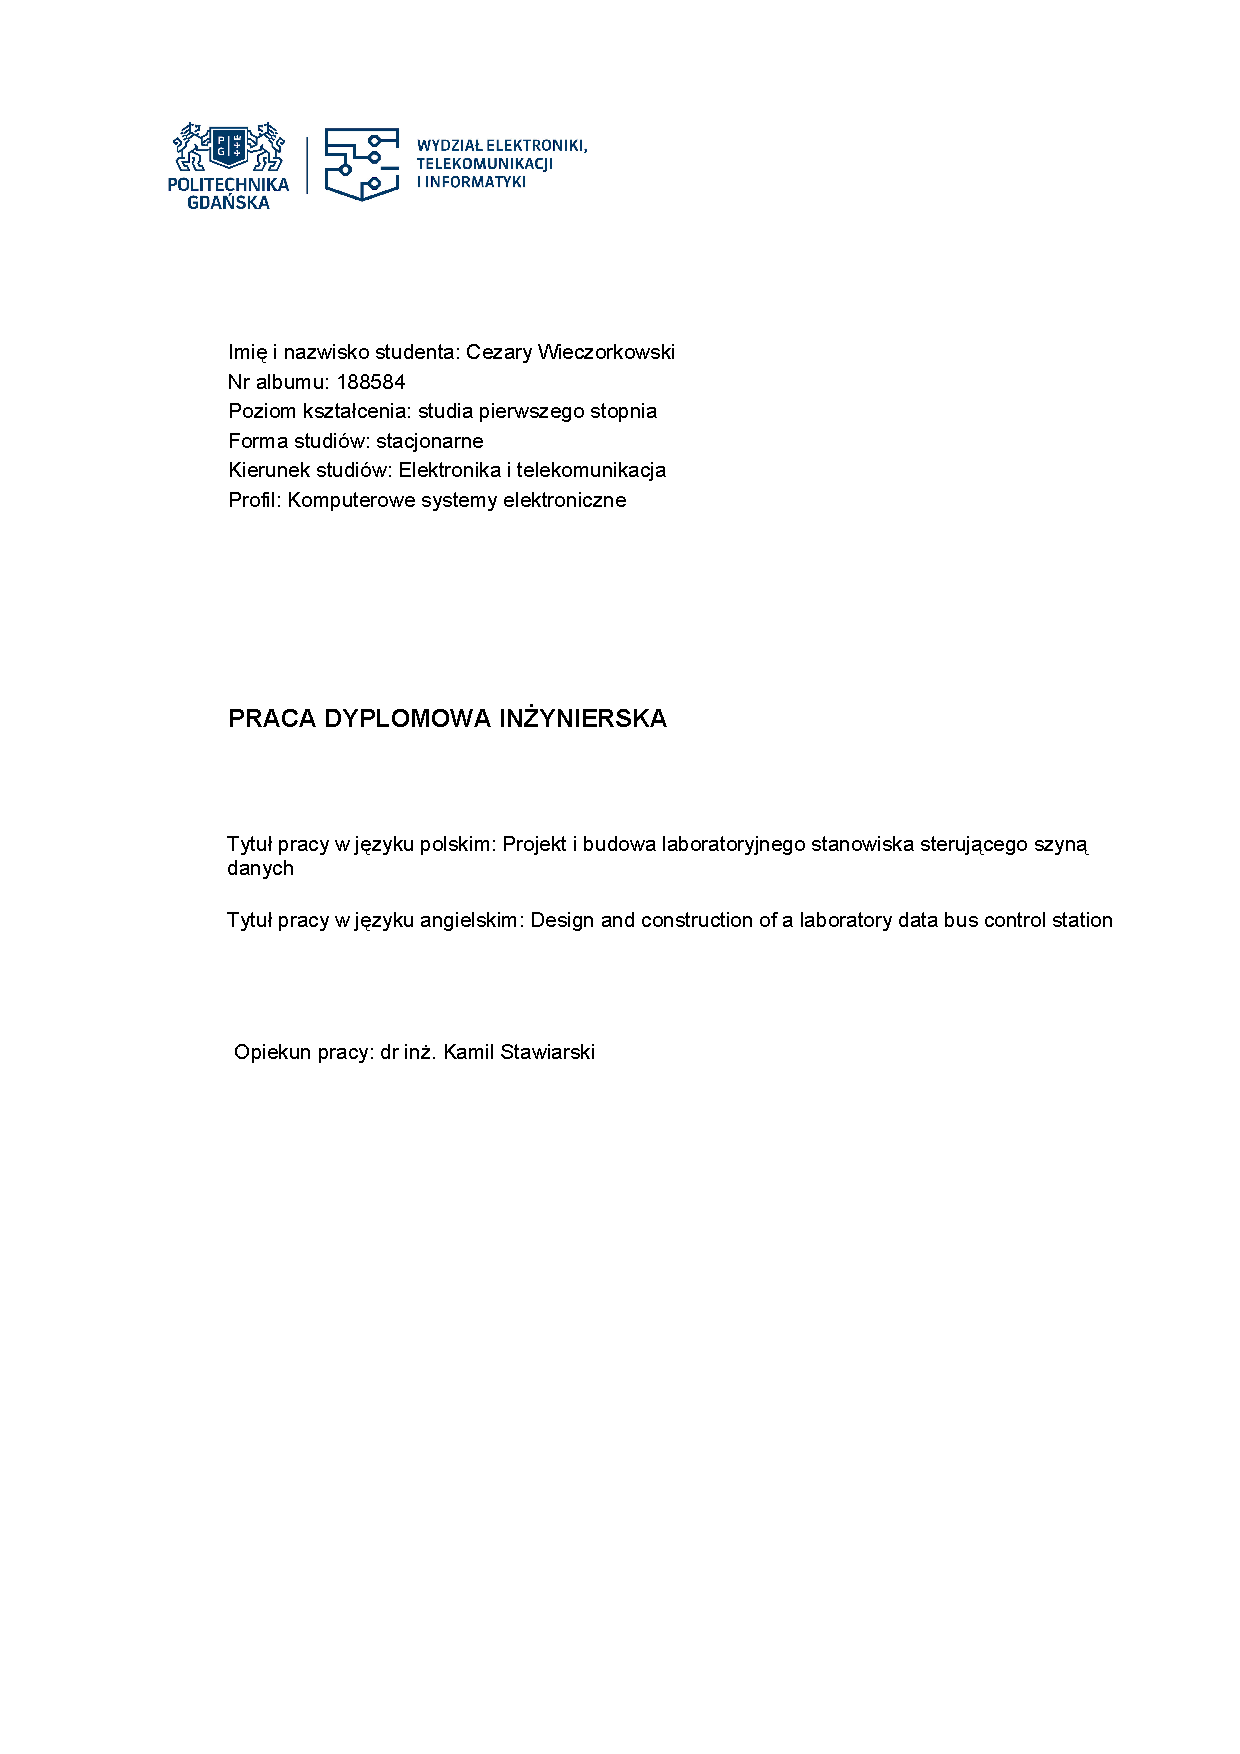
\includepdf[pages=1]{title_page.pdf}
\thispagestyle{empty}
\cleardoublepage

\subfile{abstract}
\cleardoublepage

\tableofcontents
\newpage
\subfile{skroty}
\cleardoublepage

\subfile{wstep/wstep}
\clearpage
\subfile{analiza/analiza}
\clearpage
\subfile{koncepcja/koncepcja}
\clearpage
\subfile{implementacja/implementacja}
\clearpage
\subfile{testy/testy}
\clearpage
\subfile{podsumowanie/podsumowanie}

\clearpage
\printbibliography
\addcontentsline{toc}{section}{Bibliografia}
\newpage
\listoffigures
\addcontentsline{toc}{section}{Spis rysunków}
\newpage
\listoftables
\addcontentsline{toc}{section}{Spis tabel}
\end{document}
